\documentclass{beamer}
\usepackage{tikz}
\usepackage{verbatim}
\usepackage{movie15}
\usetheme{Warsaw}
\title{Intersection Management with Constraint-Based Reservation
Systems}
\date{}

\newcommand{\goal}{find a way to make all types of vehicles to
achieve the benefits (better than traffic signal, may not be as good
as 100\% fully autonomous vehicles)}

\defbeamertemplate*{footline}{shadow theme}
{%
  \leavevmode%
  \hbox{\begin{beamercolorbox}[wd=.5\paperwidth,ht=2.5ex,dp=1.125ex,leftskip=.3cm plus1fil,rightskip=.3cm]{author in head/foot}%
    \usebeamerfont{author in head/foot}\insertframenumber\hfill\insertshortauthor
  \end{beamercolorbox}%
  \begin{beamercolorbox}[wd=.5\paperwidth,ht=2.5ex,dp=1.125ex,leftskip=.3cm,rightskip=.3cm plus1fil]{title in head/foot}%
    \usebeamerfont{title in head/foot}Tsz-Chiu Au, Shun Zhang, and Peter
Stone%
  \end{beamercolorbox}}%
}

\begin{document}

\begin{frame}
\titlepage
Tsz-Chiu Au\footnotemark[2], Shun Zhang\footnotemark[1], and Peter
Stone\footnotemark[1]
\footnotetext[1]{Department of Computer Science. The University of
Texas at Austin.}
\footnotetext[2]{School of Electrical and Computer Engineering.
Ulsan National Institute of Science and Technology.
South Korea.}
\end{frame}

\section{Introduction}

\subsection{Autonomous Intersection Management}

\begin{frame}{Intersection Management: Present and Future}
\begin{columns}[c]
	\column{.6\textwidth}
		\begin{itemize}
		\item Today's transportation infrastructure is designed for
		human drivers.
		\item In the future: \textbf{Autonomous Intersection
		Management}.\\
		Utilize the capacity of autonomous vehicles, as a large
		multi-robot system, to improve traffic in transportation
		systems.
		\end{itemize}
		
	\column{.4\textwidth}
		\includegraphics[width=0.8\textwidth]{intersection.jpg}
		\hfill
		\includegraphics[width=0.8\textwidth]{42.png}
\end{columns}
\end{frame}

\begin{frame}{Previous Work: Autonomous Intersection Management}
\begin{columns}[c]
	\column{.4\textwidth}
		\begin{center}
		\begin{figure}
		\includemovie[
		poster=./aim.png,
		text={Click to start}
		]
		{4cm}{3cm}{./fcfs-insanity.avi}
		\end{figure}
		\end{center}
				
	\column{.6\textwidth}
		\begin{itemize}
		\item Multi-agent approach.\\\cite{bib:Dresner08Multiagent}.
		\item First Come First Serve (FCFS). Use Grid-Based Collision Detection.\pause
		\item Dramatically reduce the traffic delay.
		\item Reduce the overhead of fuel consumption by approximately
		two thirds.
		\end{itemize}
\end{columns}
\end{frame}

\begin{frame}{Grid-Based Collision Detection}
	\includegraphics[width=\textwidth]{grids.png}
\end{frame}

\section{Semi-Autonomous Intersection Manangement}

\subsection{Motivation}

\begin{frame}{Sharing the Road with Human Drivers}
\begin{columns}[c]
\column{.6\textwidth}
\begin{itemize}
\item AIM is designed for the time when vehicles are autonomous.
\item Autonomous vehicles won't displace manual-controlled vehicles in
one day. Some people enjoy driving.\pause
\item One solution: FCFS-Signal = First-Come First-Served Policy +
Traffic Signals \cite{bib:Dresner08Multiagent}
\end{itemize}
\column{.4\textwidth}
\includegraphics[width=\textwidth]{fcfs-light-1.png}
\hfill
\includegraphics[width=\textwidth]{fcfs-light-2.png}
\end{columns}
\end{frame}

\begin{frame}{Observation}
\begin{itemize}
\item This ignores the possible equipments of human-driven vehicles
(e.g.\ cruise control).
\item The desirable performance is reached when 90\% of the vehicles
are fully autonomous.\pause

\includegraphics[width=0.6\textwidth]{bad_human.png}
\end{itemize}
\end{frame}

\begin{frame}{Observation}
\textbf{Goal}: \goal.
\end{frame}

\subsection{Semi-Autonomous Vechiles}

\begin{frame}{Definition}
\textbf{Semi-autonomous vehicles}: vehicles with limited autonomous
driving and wireless communication capabilities.\pause
% spectrum with H and A on both ends

\hfill

They are able to follow a \textit{limited number} of predictable
trajectories at intersections more precisely than human drivers.
\end{frame}

% TODO use graphics?
\begin{frame}{Set of Equipments}
\begin{itemize}
\item \textbf{Communication Device (Com)}:
a component in a vehicle's on-board electronic system that enables the
vehicle to wirelessly communicate with the transportation
infrastructure including the IM.\pause
% no need to change the mechanism
\item \textbf{Simple Cruise Control (CC)}:
An optional speed control subsystem in vehicles' drivetrain that
automatically controls the vehicle speed by taking over the throttle
of the vehicles.\pause
\item \textbf{Adaptive Cruise Control (ACC)}:
an advanced cruise control system that automatically adjusts the speed
of a vehicle in order to maintain a certain distance from vehicles
ahead.
\end{itemize}
\end{frame}

% FIXME not clear? not abbreviations..
\begin{frame}{Type of Semi-Autonomous Vehicles}
\begin{tabular}{|c|c|c|c|}
  \hline
  Vehicle Type & Communication & Cruise & Adaptive \\
               & Device & Control & Cruise Control \\
  \hline
  SA-ACC & X & X & X  \\
  \hline
  SA-CC & X & X &  \\
  \hline
  SA-Com & X & &  \\
  \hline
\end{tabular}
\end{frame}

\subsection{Interaction Model}

\begin{frame}{Interaction Model}
For safety, we need to define a simple and clean interface between the
human driver and the vehicle.\pause

\includegraphics[width=\textwidth]{figures/interaction}
\end{frame}

\subsection{Constraint-Based Reservation Systems}

\begin{frame}{Constraint-Based Reservation}
We turn AIM into a \emph{constraint-based reservation system}, which
allows vehicles to make reservations in terms of constraints over
\begin{itemize}
\item their driving profiles such as their arrival time and arrival velocity
\item the relationships with other vehicles.
\end{itemize}
\end{frame}

\begin{frame}{Basic Elements}
\begin{itemize}
\item{\bf Intention}: The direction in which the vehicle intends to
move.\pause
\item{\bf Vehicle Type}: The type of vehicle.\pause
\item{\bf Entry Condition}: The condition under which the vehicle will
enter the intersection.\pause
\item{\bf Acceleration Profile List}: The list of possible
acceleration schedules from among which the vehicle will choose one to
follow during the traversal of the intersection.
\end{itemize}
\end{frame}

\begin{frame}{Constant-Velocity Request}
\begin{itemize}
\item ${\sf Intent} = ( l_1 \vee l_2 \vee \ldots \vee l_n )$
in which $l_i$ is a possible lane from which the vehicle 
exits the intersection;
\item ${\sf Type}$ is the vehicle type;
\item ${\sf Entry} = (( l'_1 \vee l'_2 \vee \ldots \vee l'_n ), [t_1,\ t_2], [v_1,\ v_2])$
is the entry statement; and
\item ${\sf AP} = ( \langle (t_1, 0) \rangle )$
\end{itemize}

For the performance of Simple Cruise Control.
\end{frame}

\begin{frame}{Whole-Row Request}
\begin{itemize}
\item ${\sf Intent} = ( l_1 \vee l_2 \vee \ldots \vee l_n )$ $l_i$ is a possible lane from which the vehicle exits the intersection;
\item ${\sf Type}$ is the vehicle type;
\item ${\sf Entry} = (( l'_1 \vee l'_2 \vee \ldots \vee l'_n ), [t_1,\ t_2], [v_1,\ v_2])$ is the entry statement; and
\item ${\sf AP}$ is the acceleration profile list, and may not be
provided.
\end{itemize}

For the performance of Communication Device.
\end{frame}

\begin{frame}{Anchor Request}
Semi-autonomous vehicles with adaptive cruise control can use a special
constraint-based request called \emph{anchor requests} to make
reservations.\pause

\hfill

An anchor request is $\langle {\sf Type}, \texttt{vin},
d \rangle$
\end{frame}

\begin{frame}[fragile]{A General Request}
In Lisp syntax,

\begin{small}
\begin{verbatim}
(cc-profile (v verror angle)
  (is-auto-speed-control)
  (not is-auto-steering)
  (< velocity (+ v verror))
  (> velocity (- v verror))
  (< steer-angle angle) (> steer-angle -angle))
\end{verbatim}
\end{small}
\end{frame}

\section{Evaluations}

\begin{frame}{Evaluation on AIM (Previous Work)}
\includegraphics[width=0.8\textwidth]{old_result.png}

\cite{bib:Dresner08Multiagent}
\end{frame}

\begin{frame}{Goal}
Recall, our \textbf{goal}: \pause \goal.
\end{frame}

\begin{frame}{Implementation}
\begin{tabular}{|c|c|c|c|}
  \hline
  Vehicle Type & Communication & Cruise & Adaptive \\
               & Device & Control & Cruise Control \\
  \hline
  SA-ACC & X & X & X  \\
  \hline
  SA-CC & X & X &  \\
  \hline
  SA-Com & X & &  \\
  \hline
\end{tabular}

\hfill

For each type of vehicle - always try the most \emph{advanced} type of
request first.
\end{frame}

\begin{frame}{Evaluation on SemiAIM}
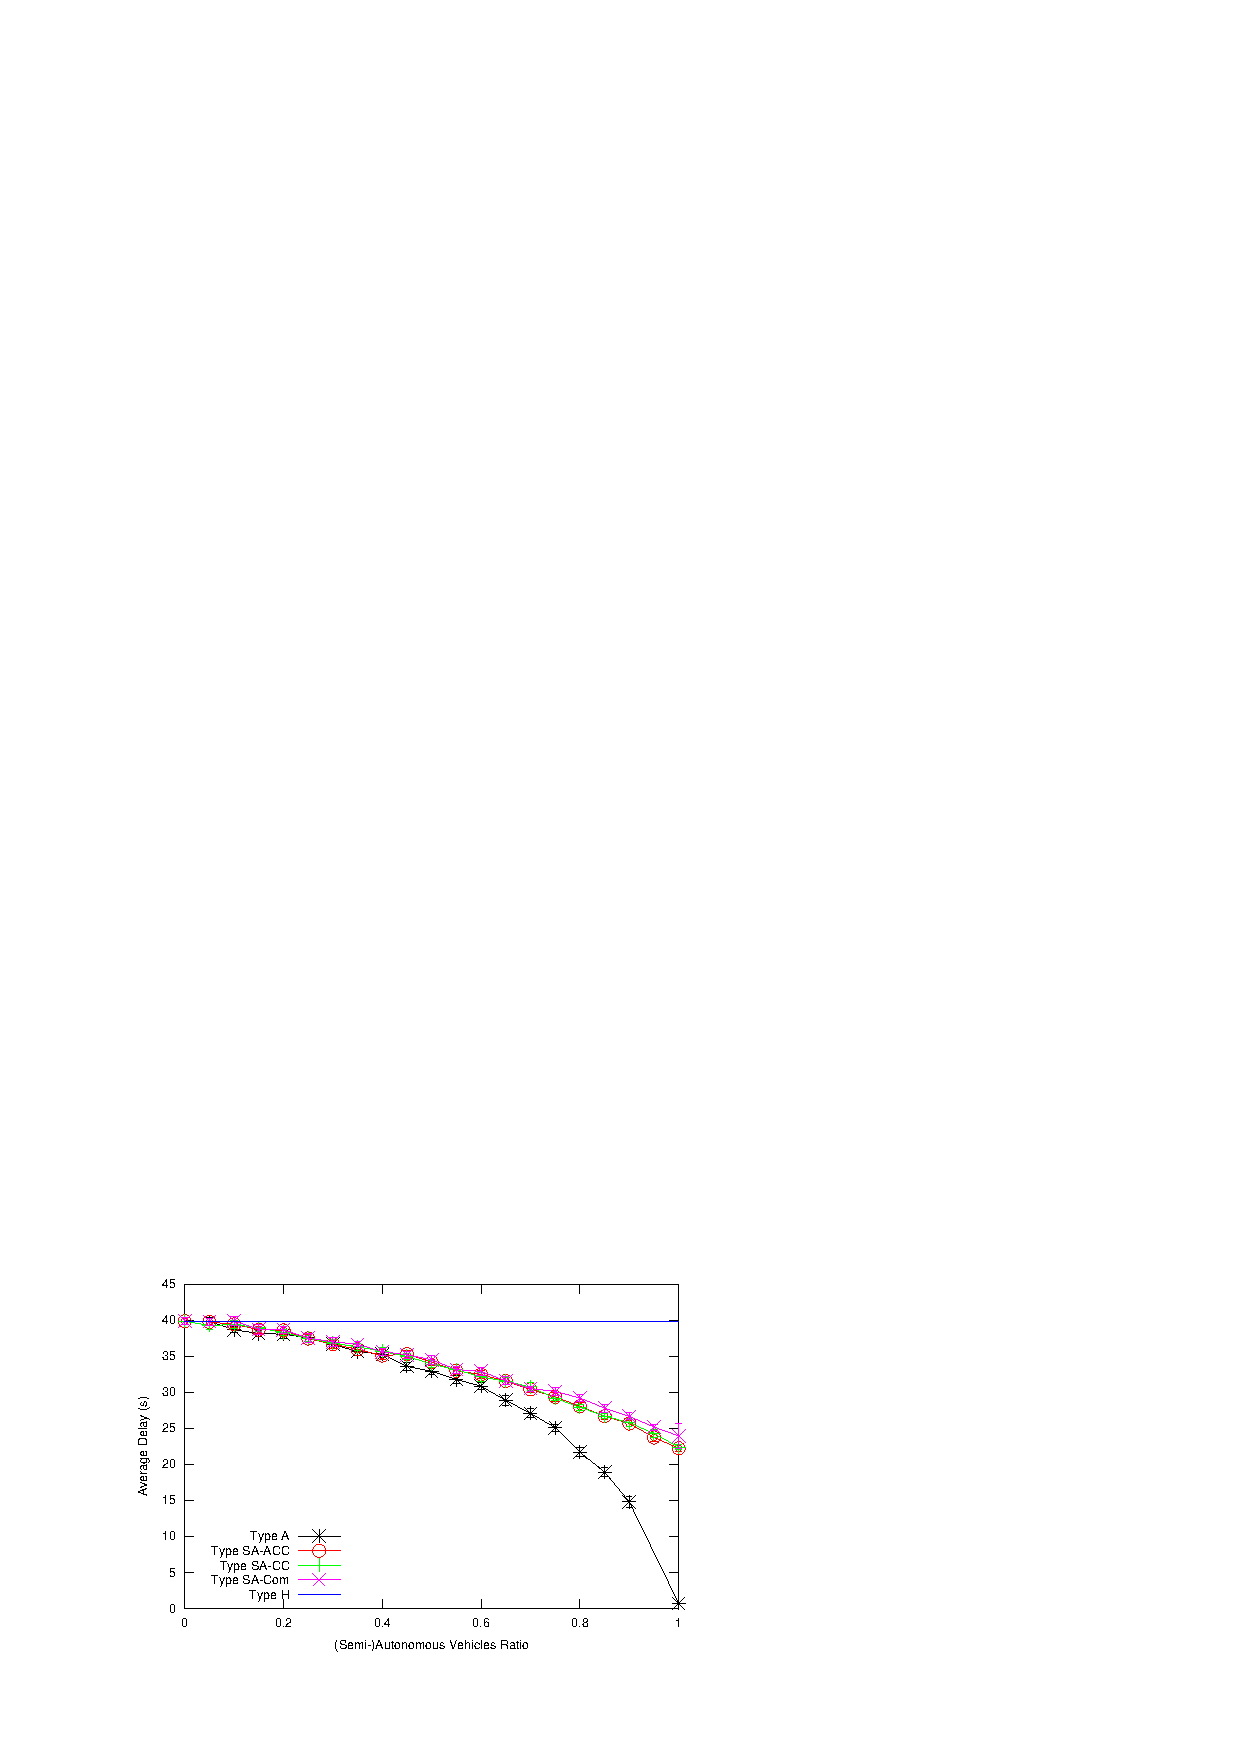
\includegraphics[width=0.9\textwidth]{figures/figure_1.pdf}

(Semi-)Autonomous vehicles vs. Human-Driven vehicles. Traffic
level = 360 vehicles/lane/hour.
\end{frame}

\begin{frame}{Evaluation on SemiAIM}
\begin{columns}[c]
	\column{.6\textwidth}
	\includegraphics[width=\columnwidth]{figures/figure_4.pdf}

	\column{.4\textwidth}
	\small
	\begin{tabular}{|c|c|c|}
    \hline
    Type H&  SemiAuto &    Type A\\
    \hline
    90\% &      \ 9\% &   \ 1\% \\
    \hline
    87\% &     11\% &    \ 2\% \\
    \hline
    84\% &     13\% &    \ 3\% \\
    \hline
     ...&   ...&   ...\\
    \hline
    \ 0\%&     69\% &  31\% \\
    \hline
	\end{tabular}

\end{columns}

\hfill

The average delay according to a deployment schedule. Traffic level =
360 vehicles/lane/hour.
\end{frame}

% FIXME SemiAIM not defined
\begin{frame}{Evaluation on SemiAIM}
\begin{columns}[c]
	\column{.6\textwidth}
	\includegraphics[width=\columnwidth]{figures/figure_3.pdf}

	\column{.4\textwidth}
	\small
	\begin{tabular}{|c|c|c|}
    \hline
     Type H&  SemiAuto &    Type A\\
    \hline
     10\%&     85\%&   \ 5\% \\
    \hline
     10\%&     80\%&  10\% \\
    \hline
     10\%&     75\%&  15\% \\
    \hline
      ...&  ... &  ...\\
    \hline
     10\%&       5\%&  85\% \\
    \hline
	\end{tabular}
\end{columns}

\hfill

The average delay according to a deployment schedule. Traffic level =
360 vehicles/lane/hour.
\end{frame}


\section{Conclusion}

\begin{frame}{Related Works}
\begin{itemize}
\item The main context of our work is an extension to the FCFS policy
proposed by Dresner and Stone \cite{bib:Dresner08Multiagent}.
\item Similar to the analysis of adaptive cruise control performance
by Jerath and Brennan \cite{bib:Jerath10adaptive}.
\item Part of a series of robotic car competitions such as the
\emph{DARPA Grand Challenges}~\cite{DARPAGrandChallenge}.
\item Jointly optimizing
autonomous vehicles and road infrastructure, for example, the PATH
program~\cite{bib:Shladover91Automated}.
\item Vehicle-to-Vehicle (V2V) forms of autonomous intersection
management~\cite{naumann97:intersection, ATT08-vanmiddlesworth}.
\end{itemize}
\end{frame}

\begin{frame}{Conclusion}
\begin{columns}[c]
\column{.4\textwidth}
	\includegraphics[width=\textwidth]{aim.png}
\column{.6\textwidth}
	\begin{itemize}
	\item SemiAIM is the first multiagent protocol to enable smooth
	interactions between human-driven, fully autonomous, and
	semiautonomous vehicles.\pause
	\item Our experiments showed that our system can greatly decrease
	traffic delay when most vehicles are semiautonomous, even when few
	(if any) are fully autonomous.
	\end{itemize}
\end{columns}
\end{frame}

\begin{frame}{Bibliography}
\tiny{\bibliographystyle{apalike}
\bibliography{bib/ref,bib/chiu,bib/intelligent_vehicles,bib/intersection,bib/peter}}
\end{frame}

\end{document}
